\section{Theorie}
\label{sec:Theorie}

\subsection{Einleitung}

Im folgenden Experiment werden diverse Schaltungen mit Operationsverstärkern
aufgebaut und ausgemessen um ein besseres Verständnis von diesen zu erhalten.
Dazu werden zunächst einige theoretische Grundlagen in den folgenden Abschnitten
bereitgestellt.

\subsection{Funktionsweise und Kenngrößen eines Operationsverstärkers}

Ein Operationsverstärker ist im Wesentlichen ein Differenzverstärker, der in der Lage ist, eine Eingangsspannungsdifferenz
mit Hilfe zweier Betriebsspannungen unterschiedlichen Vorzeichens zu verstärken.
Die dafür notwendige Beschaltung ist in Abbildung \ref{fig:OPVGrund} schematisch dargestellt.

\begin{figure}
  \centering
  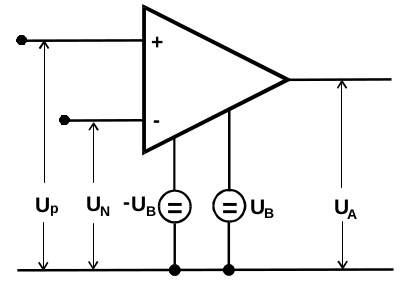
\includegraphics[height=5cm]{ImmerDieseNorweger/OPVGrund.png}
  \caption{Schematische Darstellung der grundlegenden Beschaltung eines Operationsverstärkers \cite{anleitung}.}
  \label{fig:OPVGrund}
\end{figure}

Die Spannung $U_\text{p}$, die am sogenannten nicht-invertierenden Eingang $(+)$ anliegt, geht positiv
in die Ausgangsspannung $U_\text{A}$ ein und ist entsprechend mit ihr in Phase, während die Spannung $U_\text{N}$,
welche am invertierenden Eingang $(-)$ anliegt, abgezogen wird und entsprechend gegenphasig zur Ausgangsspannung ist.
Innerhalb des sogenannten Aussteuerungsbereichs, welcher durch die Betriebsspannungen $U_\text{B}$ gegeben ist, gemäß
\begin{align}
  -U_\text{B} < U_\text{A} < U_\text{B},
\end{align}
gilt für die Ausgangsspannung $U_\text{A}$ ein linearer Zusammenhang
\begin{align}
  U_\text{A} = V \left( U_\text{p} - U_\text{N} \right),
\end{align}
wobei $V$ der Verstärkungsfaktor ist. Außerhalb dieses Bereichs geht $U_\text{A}$ in eine
Sättigung und nähert sich den Werten $\pm U_\text{B}$ an.
Die soeben beschriebene Kennlinie eines Operationsverstärkers ist in Abbildung \ref{fig:kennlinieOPV}
noch einmal skizziert.

\begin{figure}
  \centering
  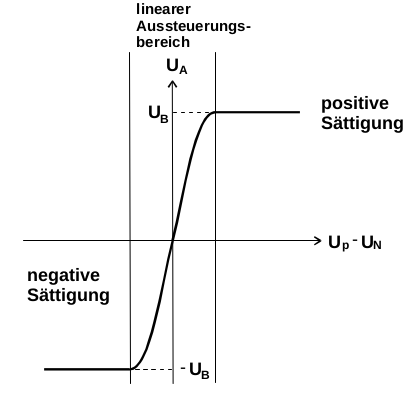
\includegraphics[height=7cm]{ImmerDieseNorweger/kennlinieOPV.png}
  \caption{Schematische Kennlinie eines Operationsverstärkers im und außerhalb des Aussteuerungsbereichs \cite{anleitung}.}
  \label{fig:kennlinieOPV}
\end{figure}

Es ist für das Verständnis diverser Kenngrößen praktisch diese zunächst an einem idealen Operationsverstärker
einzuführen und sie anschließend auf entsprechende endliche Werte an einem
realen Operationsverstärker zu übertragen. Die Eingangswiderstände $R_\text{e,p}$ und $R_\text{e,N}$
und die Leerlaufverstärkung $V$ beim idealen Operationsverstärker gehen gegen unendlich während der
Ausgangswiderstand $R_\text{a}$ gegen Null geht. Entsprechend sind beim realen Operationsverstärker
$R_\text{e,p}$ und $R_\text{e,N}$ groß und $R_\text{a}$ klein, während die Leerlaufverstärkung
$V$ groß und außerdem frequenzabhängig ist. Die Tatsache, dass die Größen alle endlich sind hat das
Auftreten mehrerer Störeffekte am realen Operationsverstärker zur Folge.

So wird aufgrund von Unsymmetrien der Verstärkerkanäle beispielsweise auch bei zwei
gleichen Eingangsspannungen noch eine endliche Ausgangsspannung beobachtet. Die sogenannte Gleichtaktverstärkung
bemisst dieses Störsignal und ist gegeben durch den Quotienten zwischen Ausgangsspannung und
Gleichtakteingangsspannung
\begin{align}
  V_\text{Gl} = \frac{U_\text{A}}{U_\text{Gl}}.
\end{align}
Da die Eingangswiderstände endlich sind entstehen Störströme an den Verstärkereingängen.
Entsprechend wird der mittlere Eingangsruhestrom
\begin{align}
  I_\text{B} = \frac12 \left( I_\text{p} + I_\text{N} \right)
\end{align}
und zudem auch, aufgrund von Unsymmetrien der Verstärkerkanäle, der sogenannte
Eingangsoffsetstrom
\begin{align}
  I_0 = I_\text{p} - I_\text{N}
\end{align}
definiert. Letzterer wird bei verschwindenden Eingangsspannungen $U_\text{p} = U_\text{N} = 0$ gemessen.

Obwohl die Gleichtaktverstärkung bei der Gleichtakteingangsspannung $U_\text{Gl} = 0$ verschwindet
kann am realen Operationsverstärker noch eine Ausgangsspannung detektiert werden. Entsprechend wird die sogenannte
Offsetspannung $U_0$ definiert. Sie ist abhängig von Temperatur, Frequenz und den Betriebsspannungen und gegeben
durch die Eingangsspannungsdifferenz, welche gerade die Ausgangsspannung $U_\text{A} = 0$ liefert, gemäß
\begin{align}
  U_0 = U_\text{p} - U_\text{N}.
\end{align}

Die aufgezählten Kenngrößen geben an, wie gut ein realer Operationsverstärker arbeitet. Beim idealen
Operationsverstärker sind sie selbstverständlich alle Null. In den nächsten Abschnitten werden verschiedene
Beschaltungen von Operationsverstärkern mit unterschiedlichen Wirkungen präsentiert.

\subsection{Linearverstärker}

Um den Operationsverstärker als Linearverstärker verwenden zu können muss zunächst eine Möglichkeit gefunden werden,
den Verstärkungsfaktor zu reduzieren. Das ist nötig, da der Leerlaufverstärkungsfaktor bei realen Operationsverstärkern
sehr hoch ist, etwa in der Größenordnung $10^5$, und der Aussteuerungsbereich, dessen Breite sich ja antiproportional
zum Verstärkungsfaktor verhält, entsprechend klein. Damit wird der Sättigungsbereich, welcher ja beim Linearverstärker
gemieden werden sollte, bereits bei kleinen Eingangsspannungsdifferenzen erreicht.
Eine Gegenkopplungsschaltung, wie sie in Abbildung \ref{fig:gegenkopplung} zu sehen ist, löst dieses Problem.

\begin{figure}
  \centering
  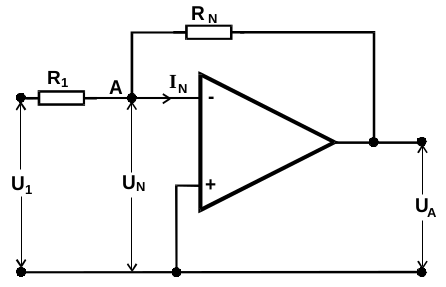
\includegraphics[height=5cm]{ImmerDieseNorweger/gegenkopplung.png}
  \caption{Schematischer Schaltplan für den gegengekoppelten invertierenden Linearverstärker\cite{anleitung}.}
  \label{fig:gegenkopplung}
\end{figure}

Ein Teil der Ausgangsspannung wird zurück auf den invertierenden Eingang gegeben, sodass die Eingangsspannungsdifferenz
und schließlich auch die Ausgangsspannung reduziert wird. Dadurch wird insgesamt ein geringerer Verstärkungsfaktor abhängig von
den eingebauten Widerständen $R_1$ und $R_\text{N}$ erreicht. Mit den Kirchhoffschen Regeln lässt sich für den idealen
Operationsverstärker, für welchen $U_\text{N}$ und $I_\text{N}$ gegen Null gehen, der Verstärkungsfaktor
\begin{align}
  V_\text{lin,ideal} = \frac{U_\text{A}}{U_\text{1}} = \frac{R_\text{N}}{R_1}
\end{align}
herleiten. Dieser hängt nur von der äußeren Beschaltung des Operationsverstärkers und nicht von ihm selbst ab.
Beim realen Operationsverstärker kann mit der Korrektur, dass die Leerlaufverstärkung endlich ist, der
Verstärkungsfaktor
\begin{align}
  V' \approx \left( \frac1{V} + \frac{R_\text{N}}{R_1} \right)^{-1}
\end{align}
hergeleitet werden, wobei $V$ wieder die Leerlaufverstärkung ist. Für den Fall eines großen Widerstandsquotienten
\begin{align}
  \frac{R_\text{N}}{R_1} >> V
\end{align}
geht der reale in den idealen Wert über und der Verstärkungsfaktor ist wieder unabängig von dem Operationsverstärker selbst.
Werden also die Widerstände entsprechend gewählt, so arbeitet der Operationsverstärker stabiler gegen Temperaturschwankungen
und Exemplarstreuungen, sofern die äußere Beschaltung gegenüber diesen stabil ist.




\subsection{Fehlerrechnung}

Für die Fehlerfortpflanzung bei Gleichungen mit $N$ fehlerbehafteten Größen
wird jeweils die Formel zur Gaußschen Fehlerfortpflanzung

\begin{equation*}
  \sigma = \sqrt{\sum_{i=1}^{N}\biggl(\frac{\partial f(x_{\g{i}})}{\partial x_{\g{i}}}
  \sigma_{\g{i}}\biggr)^2}
\end{equation*}
mit der jeweiligen Funktion $f(x_{\g{i}})$, den Messgrößen $x_{\g{i}}$ und den
zugehörigen Fehlern $\sigma_i$ verwendet.
Zur Berechnung des arithmetischen Mittels von $N$ Messwerten wird jeweils die
Formel

\begin{equation*}
  \bar{x} = \frac{1}{N}\sum_{i=1}^{N}x_{\g{i}}
\end{equation*}
mit den Messwerten $x_i$ benutzt.
Die Standardabweichung des Mittelwerts wird jeweils mit der Gleichung

\begin{equation*}
  \bar{\sigma} = \sqrt{\frac{1}{N-1}\sum_{i=1}^{N}(x_{\g{i}} - \bar{x})^2}
\end{equation*}
mit den $N$ Messwerten $x_i$ berechnet.


\cite{anleitung}
